\documentclass[a4paper,12pt]{article}
\usepackage{graphicx}
\usepackage{amsmath, amssymb}
\usepackage{hyperref}
\usepackage{tikz}
\usepackage{float}  
\usepackage{placeins}
\usepackage[backend=biber, style=numeric, citestyle=ieee]{biblatex}

\addbibresource{references.bib}


\title{Centripetal Force: Technical Paper for Activity 3}
\author{Janelle Lastimado \\
John Paul Memoracion \\ 
Nikki Shane Mercado \\
Gian Myrl Renomeron}
\date{February 20, 2025}

\begin{document}

\maketitle

\begin{abstract}
    This experiment delves into the concept of centripetal force and its function to maintain circular motion. A spinning cork attached to a hanging mass was used to study motion with the correlation of mass, velocity, radius, and centripetal force. Theoretical calculations were obtained from cork measurements using Newton's second law of motion. The percentage difference between these values was compared to determine the accuracy of the experiment. External forces and human error were taken into account. The results give one an understanding of the concepts involved in circular motion and what conditions are necessary to achieve uniform rotation.
\end{abstract}

\section{Introduction}
Centripetal force is the force that positions the object's motion in circular manner, always centripetally directed into the circle's center. It does not alter the object's speed but modifies its direction, causing centripetal acceleration.\cite{LucasGhose2024} The acceleration is provided by \(a = v² / r \), where v represents constant speed and r represents the radius of the circular path. Based on Newton's second law of motion, centripetal force is given by F = ma, or alternatively, \( F = mv² / r\) for an object traveling at constant speed in a circular motion.\cite{CentripetalForce}\\

This experiment is set to explore the relationship between centripetal force and the radius of the circular path. By changing the radius and taking the time for a fixed number of revolutions, the centripetal force can be derived and studied. A cork system is employed, in which the force is counterbalanced by a hanging mass. The system also supports adjusting the radius and noting down the resulting changes to keep the mass at a position of equilibrium. The aim is to verify experimentally the centripetal force, mass, velocity, and radius relationship, and also compare the result from experiments to the predictions obtained from theory.
\section{Materials and Methodology}


\subsection{Materials}
Below are the list of materials used in the experiment
\begin{itemize}
    \item Pen case
    \item Fishline
    \item Paper clip
    \item Platform balance
    \item Stopwatch
    \item Cork
    \item Set of Masses
\end{itemize}

\subsection{Methodology}
The goal of this experiment is to determine the centripetal force acting on a rotating object. Figure \ref{fig:setup} shows the setup of the experiment.


\paragraph{Procedure}

\begin{figure}[]
    \centering
    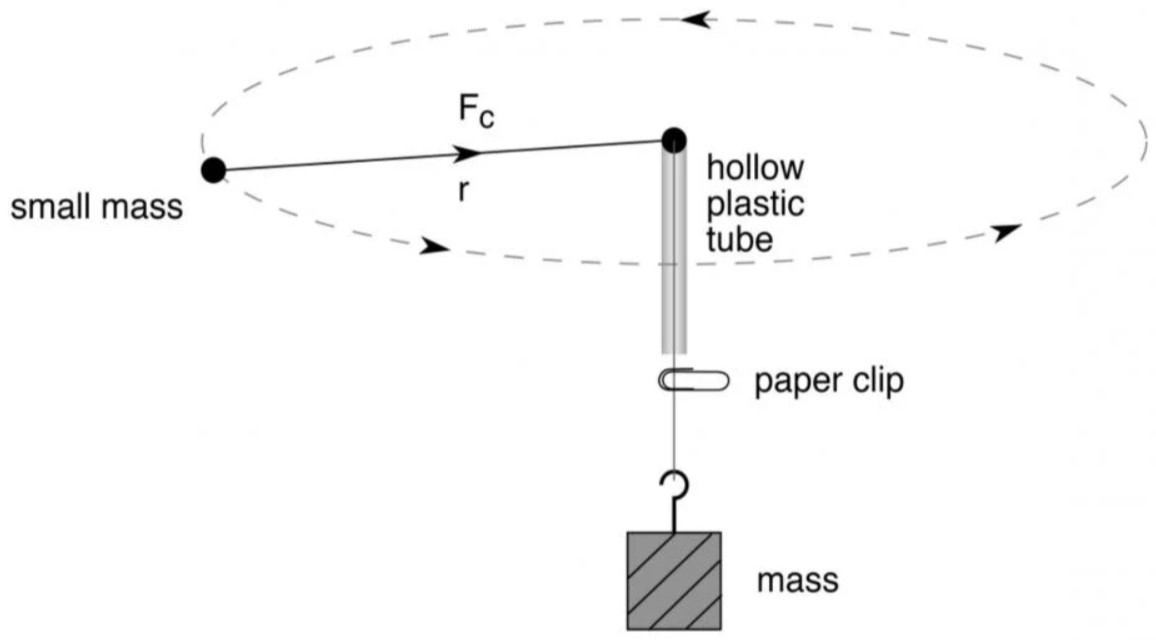
\includegraphics[width=1\textwidth]{experiment_setup.png}
    \caption{Experimental setup}
    \label{fig:setup}
\end{figure}

\begin{enumerate}
    \item Measure the mass of the cork. Hang a 50 g mass on one end of the fishline (this serves as the theoretical value for the centripetal force). Insert the other end into the pen case. The cork must be tied to this end. Support the mass with one hand and hold the pen case in the other.
    \item Fasten a paper clip just below the bottom of the pen case. Whirl the cork by revolving the pen case. Slowly release the 50 g mass and adjust the speed of revolution so that the paper clip stays in place.
    \item Next, grasp the string at the bottom of the pen case to mark the position of the string while the cork is moving. With the string in this position, measure the radius \textbf{r}.
    \item For the same mass change the radius of the rotation first to the smaller value and then to a larger value. Observe the corresponding change to maintain the mass at the stationary position.
\end{enumerate}


\section{Results and Discussion}
Below is the data and result of the experiments. The small mass is 0.05 kg. The theoretical value used is 0.49 \textbf{N}, which was calculated using mass times gravity.

\subsection{Experiment 1: Mass constant, Force varies}
\begin{table}[h]
    \centering
    \renewcommand{\arraystretch}{1.2}
    \makebox[\textwidth]{ 
        \begin{tabular}{|c|c|c|c|c|c|c|}
            \hline
            \textbf{Trial} & \textbf{m (kg)} & \textbf{r (m)} & \textbf{Period (s)} & \textbf{$v$ (m/s)} & \textbf{$v^2$ (m/s)} & \textbf{F (N)} \\
            \hline
            1 & 0.05 kg & 0.15 m & 0.65 s & 1.45 m/s & 2.10 m/s & 0.7 N \\
            2 & 0.05 kg & 0.20 m & 0.77 s & 1.61 m/s & 2.6 m/s & 0.65 N \\
            3 & 0.05 kg & 0.30 m & 0.9 s & 2.09 m/s & 4.39 m/s & 0.73 N \\
            \hline
        \end{tabular}
    }
    \caption{Results of the Experiment}
    \label{table:exp}
\end{table}

As one can see in table \ref{table:exp}, constant small mass with varying radius produced varying period and velocity. From these values, period increased as the radius increased. The total time for each trials are 16.25, 19.25 and 22.5, respectively. These values are rounded up to the nearest hundredth. The average centripetal force (experimental values) is 0.69. The Percent difference (percent diff between the experimental (Fexp) and theoretical (F) centripetal force) is calculated using this formula (See Figure \ref{fig:percent}):

\begin{figure}[H]
    \centering
    
\includegraphics[width=1\textwidth]{percentage.png}
    \caption{Percentage Formula}
    \label{fig:percent}
\end{figure}

The calculated percentage is \textit{33.89 \%}. If the percent difference is greater than 10\%, it means that it indicates a bad agreement. The difference can be attributed to measurement errors, timing errors, or outside influences such as friction and air resistance. Human reaction time when employing a stopwatch can influence period measurements, whereas minor errors in radius or mass affect velocity and force calculations. Furthermore, theoretical presuppositions, including uniform circular motion, cannot reflect the actual circumstances as variations in velocity or an oblique string introduce inaccuracies. Calibration and deviations in holding steady motion further play a part in the difference. These circumstances call for accuracy in measurements and conditions to prevent errors.

\section{Conclusion}

This experiment enabled us to learn the relationship between radius and velocity for centripetal force and the verification of Newton's Second Law of Motion. When we used a larger radius, we could see that period increased as well, and hence velocity and also the force applied to maintain the object in a circular motion got affected. Our results were indeed as expected, but our experimental values didn't match perfectly with the theoretical values. These might be caused by minute errors in the measurement of radius and time, delays in reaction time while using the stopwatch, or even external forces such as friction and air resistance. Despite these difficulties, the experiment served to reinforce the basic relationships among force, mass, and acceleration, demonstrating for us the significance of accurate measurements and controlled conditions in actual physics experiments.


\printbibliography

\end{document}
